

\section{Quantum Dimension}
Let $N_{ab}^{c}$ be the fusion multiplicity matrices of a TQFT
\begin{equation*}
a\times b=\sum _{c} N_{ab}^{c} c
\end{equation*}
meaning that $N_{ab}^{c}$ is the number of distinct ways that $a$ and $b$ can fuse to $c$. (In many, or even most, theories of interest all $N$ 's are either 0 or 1 ).



The quantum dimension $\mathsf{d}_{a}$ of a particle $a$ is defined as the largest eigenvalue of the matrix $[ N_{a}]_{b}^{c}$ where this is now thought of as a two dimensional matrix with $a$ fixed and $b,c$ the indices.

Show that
\begin{equation*}
\mathsf{d}_{a}\mathsf{d}_{b} =\sum _{c} N_{ab}^{c}\mathsf{d}_{c} .
\end{equation*}
We will prove this formula algebraically in Chapter 17. However there is a simple and much more physical way to get to the the result: Imagine fusing together $M$ anyons of type $a$ and $M$ anyons of type $b$ where $M$ gets very large and determine the dimension of space that results. Then imagine fusing together $a\times b$ and do this $M$ times and then fuse together all the results.

\paragraph{Answer}
We first consider the fusion of $M$ anyons of type $a$, as the Fig.\ref{fig:fusionOfMAnyonsOfTypea} shows. 
\begin{figure}[h!]
\centering
\tikzset{every picture/.style={line width=0.75pt}} %set default line width to 0.75pt        

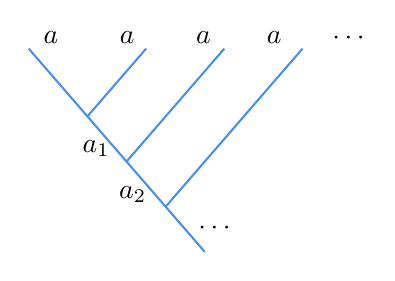
\begin{tikzpicture}[x=0.75pt,y=0.75pt,yscale=-1,xscale=1]
%uncomment if require: \path (0,115); %set diagram left start at 0, and has height of 115

%Straight Lines [id:da11955497661468573] 
\draw [color={rgb, 255:red, 74; green, 144; blue, 226 }  ,draw opacity=1 ]   (243,14.64) -- (327.81,112.57) ;
%Straight Lines [id:da6152525920183469] 
\draw [color={rgb, 255:red, 74; green, 144; blue, 226 }  ,draw opacity=1 ]   (271.29,47.31) -- (299.58,14.64) ;
%Straight Lines [id:da819418313740367] 
\draw [color={rgb, 255:red, 74; green, 144; blue, 226 }  ,draw opacity=1 ]   (290.13,69.06) -- (337.26,14.64) ;
%Straight Lines [id:da720895407290538] 
\draw [color={rgb, 255:red, 74; green, 144; blue, 226 }  ,draw opacity=1 ]   (308.97,90.82) -- (374.94,14.64) ;

% Text Node
\draw (248.71,5.06) node [anchor=north west][inner sep=0.75pt]    {$a$};
% Text Node
\draw (285.46,5.06) node [anchor=north west][inner sep=0.75pt]    {$a$};
% Text Node
\draw (267.53,57.33) node [anchor=north west][inner sep=0.75pt]    {$a_{1}$};
% Text Node
\draw (322.21,5.06) node [anchor=north west][inner sep=0.75pt]    {$a$};
% Text Node
\draw (356.28,5.06) node [anchor=north west][inner sep=0.75pt]    {$a$};
% Text Node
\draw (285.08,79.66) node [anchor=north west][inner sep=0.75pt]    {$a_{2}$};
% Text Node
\draw (323.23,96.66) node [anchor=north west][inner sep=0.75pt]    {$\cdots $};
% Text Node
\draw (387.77,5.06) node [anchor=north west][inner sep=0.75pt]    {$\cdots $};
\end{tikzpicture}
\caption{Fusion of $M$ anyons of type $a$.}
\label{fig:fusionOfMAnyonsOfTypea}
\end{figure}
Suppose the final result is $a_{M-1}$, then the dimension of fusing $M$ anyons of type $a$ to get $a_{f}$ is:
\begin{equation*}
\dim( a_{M-1}) =\sum _{a_{1} ,a_{2} \cdots a_{M-2}} N_{aa}^{a_{1}} N_{a_{1} a}^{a_{2}} \cdots N_{a_{M-2} a}^{a_{M-1}} =[( N_{a})^{M-1} ]_{a}^{a_{M-1}} .
\end{equation*}
Similarly, the fusiong of $M$ anyons of type $b$ gives
\begin{equation*}
\dim( b_{M-1}) =[( N_{b})^{M-1} ]_{b}^{b_{M-1}} .
\end{equation*}
Then the fusion of $a_{M-1}$ and $b_{M-1}$ gives
\begin{equation*}
\dim( a_{M-1} \times b_{M-1}) =\sum _{a_{M-1} b_{M-1}} [( N_{b})^{M-1} ]_{b}^{b_{M-1}} [( N_{a})^{M-1} ]_{a}^{a_{M-1}} N_{a_{M-1} b_{M-1}}^{c_{M-1}} .
\end{equation*}
In large $M$ limit, we have
\begin{equation*}
\dim( a_{M-1} \times b_{M-1}) \sim (\mathsf{d}_{b}\mathsf{d}_{a})^{M-1} .
\end{equation*}


However, if we fuse $a,b$ first to give $c$, then fuse $M$ anyons of type $c$, as the Fig.\ref{fig:FusionabFirst} shows, we get
\begin{equation*}
\dim( c_{M-1}) =[(N_{ab}^{c} N_{c} )^{M-1} ]_{c}^{c_{M-1}} N_{ab}^{c} \sim (N_{ab}^{c}\mathsf{d}_{c} )^{M-1} =\dim( a_{M-1} \times b_{M-1}) .
\end{equation*}
\begin{figure}[h!]
\centering
\tikzset{every picture/.style={line width=0.75pt}} %set default line width to 0.75pt        

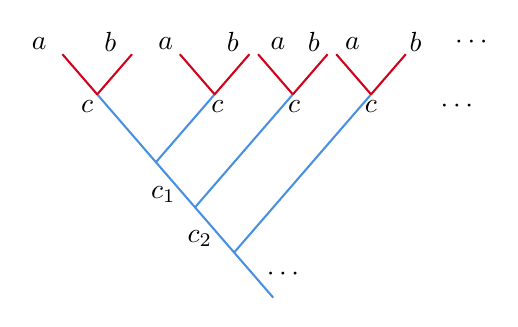
\begin{tikzpicture}[x=0.75pt,y=0.75pt,yscale=-1,xscale=1]
%uncomment if require: \path (0,137); %set diagram left start at 0, and has height of 137

%Straight Lines [id:da40929728188110026] 
\draw [color={rgb, 255:red, 74; green, 144; blue, 226 }  ,draw opacity=1 ]   (246,33.64) -- (330.81,131.57) ;
%Straight Lines [id:da9953461415866856] 
\draw [color={rgb, 255:red, 74; green, 144; blue, 226 }  ,draw opacity=1 ]   (274.29,66.31) -- (302.58,33.64) ;
%Straight Lines [id:da2994930570192573] 
\draw [color={rgb, 255:red, 74; green, 144; blue, 226 }  ,draw opacity=1 ]   (293.13,88.06) -- (340.26,33.64) ;
%Straight Lines [id:da8153796656269163] 
\draw [color={rgb, 255:red, 74; green, 144; blue, 226 }  ,draw opacity=1 ]   (311.97,109.82) -- (377.94,33.64) ;
%Straight Lines [id:da22124282289903574] 
\draw [color={rgb, 255:red, 208; green, 2; blue, 27 }  ,draw opacity=1 ]   (229.24,14.29) -- (246,33.64) ;
%Straight Lines [id:da6870786384443515] 
\draw [color={rgb, 255:red, 208; green, 2; blue, 27 }  ,draw opacity=1 ]   (262.76,14.29) -- (246,33.64) ;
%Straight Lines [id:da8781455879150906] 
\draw [color={rgb, 255:red, 208; green, 2; blue, 27 }  ,draw opacity=1 ]   (285.81,14.29) -- (302.58,33.64) ;
%Straight Lines [id:da6766518363879819] 
\draw [color={rgb, 255:red, 208; green, 2; blue, 27 }  ,draw opacity=1 ]   (319.34,14.29) -- (302.58,33.64) ;
%Straight Lines [id:da07038864761619235] 
\draw [color={rgb, 255:red, 208; green, 2; blue, 27 }  ,draw opacity=1 ]   (323.49,14.29) -- (340.26,33.64) ;
%Straight Lines [id:da6906279364980574] 
\draw [color={rgb, 255:red, 208; green, 2; blue, 27 }  ,draw opacity=1 ]   (357.02,14.29) -- (340.26,33.64) ;
%Straight Lines [id:da9480406401134733] 
\draw [color={rgb, 255:red, 208; green, 2; blue, 27 }  ,draw opacity=1 ]   (361.18,14.29) -- (377.94,33.64) ;
%Straight Lines [id:da4926866941860706] 
\draw [color={rgb, 255:red, 208; green, 2; blue, 27 }  ,draw opacity=1 ]   (394.7,14.29) -- (377.94,33.64) ;

% Text Node
\draw (236.71,35.03) node [anchor=north west][inner sep=0.75pt]    {$c$};
% Text Node
\draw (299.46,35.03) node [anchor=north west][inner sep=0.75pt]    {$c$};
% Text Node
\draw (270.53,76.33) node [anchor=north west][inner sep=0.75pt]    {$c_{1}$};
% Text Node
\draw (288.08,97.66) node [anchor=north west][inner sep=0.75pt]    {$c_{2}$};
% Text Node
\draw (326.23,115.66) node [anchor=north west][inner sep=0.75pt]    {$\cdots $};
% Text Node
\draw (213,5) node [anchor=north west][inner sep=0.75pt]    {$a$};
% Text Node
\draw (248,2) node [anchor=north west][inner sep=0.75pt]    {$b$};
% Text Node
\draw (274,5) node [anchor=north west][inner sep=0.75pt]    {$a$};
% Text Node
\draw (307,2) node [anchor=north west][inner sep=0.75pt]    {$b$};
% Text Node
\draw (328,5) node [anchor=north west][inner sep=0.75pt]    {$a$};
% Text Node
\draw (346,2) node [anchor=north west][inner sep=0.75pt]    {$b$};
% Text Node
\draw (364,5) node [anchor=north west][inner sep=0.75pt]    {$a$};
% Text Node
\draw (395,2) node [anchor=north west][inner sep=0.75pt]    {$b$};
% Text Node
\draw (336.46,35.03) node [anchor=north west][inner sep=0.75pt]    {$c$};
% Text Node
\draw (373.46,35.03) node [anchor=north west][inner sep=0.75pt]    {$c$};
% Text Node
\draw (417,4) node [anchor=north west][inner sep=0.75pt]    {$\cdots $};
% Text Node
\draw (410,35.03) node [anchor=north west][inner sep=0.75pt]    {$\cdots $};
\end{tikzpicture}
\caption{Fuse $a,b$ first to give $c$, then fuse $M$ anyons of type $c$.}
\label{fig:FusionabFirst}
\end{figure}

So we have
\begin{equation*}
\mathsf{d}_{a}\mathsf{d}_{b} =\sum _{c} N_{ab}^{c}\mathsf{d}_{c} .
\end{equation*}


\section{Fusion and Ground State Degeneracy}
To determine the ground state degeneracy of a 2-manifold in a $2+1$ dimensional TQFT one can cut the manifold into pieces and sew back together. One can think of the open "edges" or connecting tube-ends as each having a label given by one of the particle types (i.e., one of the anyons) of the theory. Really we are labeling each edge with a basis element of a possible Hilbert space. The labels on two tubes that have been connected together must match (label $a$ on one tube fits into label $\bar{a}$ on another tube.) To calculate the ground state degeneracy we must keep track of all possible ways that these assembled tubes could have been labeled. For example, when we assemble a torus as in Fig.\ref{fig:suregeringSphereToTorus}, we must match the quantum number on one open end to the (opposite) quantum number on the opposite open end. The ground state degeneracy is then just the number of different possible labels, or equivalently the number of different particle types.
\begin{figure}[h!]
\centering
\tikzset{every picture/.style={line width=0.75pt}} %set default line width to 0.75pt        

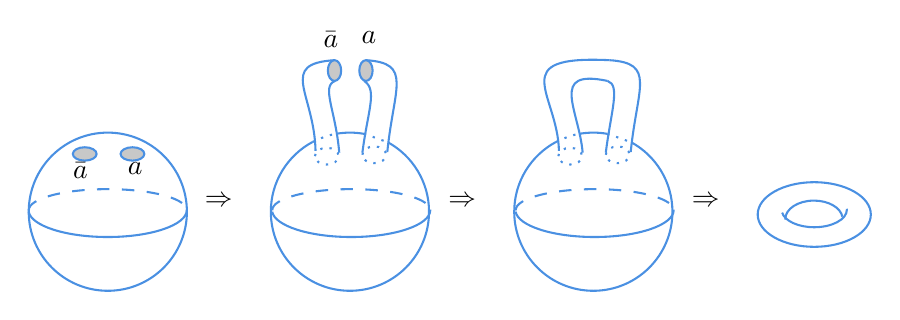
\begin{tikzpicture}[x=0.75pt,y=0.75pt,yscale=-1,xscale=1]
%uncomment if require: \path (0,133); %set diagram left start at 0, and has height of 133

%Shape: Ellipse [id:dp8367832127596704] 
\draw  [color={rgb, 255:red, 74; green, 144; blue, 226 }  ,draw opacity=1 ] (127.97,90.78) .. controls (127.97,69.73) and (145.03,52.67) .. (166.08,52.67) .. controls (187.12,52.67) and (204.18,69.73) .. (204.18,90.78) .. controls (204.18,111.82) and (187.12,128.88) .. (166.08,128.88) .. controls (145.03,128.88) and (127.97,111.82) .. (127.97,90.78) -- cycle ;
%Shape: Ellipse [id:dp3840252547503711] 
\draw  [color={rgb, 255:red, 74; green, 144; blue, 226 }  ,draw opacity=1 ][fill={rgb, 255:red, 200; green, 200; blue, 200 }  ,fill opacity=1 ] (149.22,62.94) .. controls (149.22,61.16) and (151.79,59.72) .. (154.95,59.72) .. controls (158.12,59.72) and (160.69,61.16) .. (160.69,62.94) .. controls (160.69,64.72) and (158.12,66.16) .. (154.95,66.16) .. controls (151.79,66.16) and (149.22,64.72) .. (149.22,62.94) -- cycle ;
%Shape: Ellipse [id:dp6826244717089338] 
\draw  [color={rgb, 255:red, 74; green, 144; blue, 226 }  ,draw opacity=1 ][fill={rgb, 255:red, 200; green, 200; blue, 200 }  ,fill opacity=1 ] (172.22,62.94) .. controls (172.22,61.16) and (174.79,59.72) .. (177.95,59.72) .. controls (181.12,59.72) and (183.69,61.16) .. (183.69,62.94) .. controls (183.69,64.72) and (181.12,66.16) .. (177.95,66.16) .. controls (174.79,66.16) and (172.22,64.72) .. (172.22,62.94) -- cycle ;
%Shape: Arc [id:dp6152757783671656] 
\draw  [draw opacity=0][dash pattern={on 4.5pt off 4.5pt}] (128.02,90.12) .. controls (128.02,90.07) and (128.02,90.02) .. (128.02,89.97) .. controls (128.02,84.41) and (145.03,79.9) .. (166.02,79.9) .. controls (185.99,79.9) and (202.36,83.98) .. (203.9,89.17) -- (166.02,89.97) -- cycle ; \draw  [color={rgb, 255:red, 74; green, 144; blue, 226 }  ,draw opacity=1 ][dash pattern={on 4.5pt off 4.5pt}] (128.02,90.12) .. controls (128.02,90.07) and (128.02,90.02) .. (128.02,89.97) .. controls (128.02,84.41) and (145.03,79.9) .. (166.02,79.9) .. controls (185.99,79.9) and (202.36,83.98) .. (203.9,89.17) ;  
%Shape: Arc [id:dp8238926984639989] 
\draw  [draw opacity=0] (204.13,89.83) .. controls (204.13,89.87) and (204.13,89.92) .. (204.13,89.97) .. controls (204.13,97.15) and (187.07,102.97) .. (166.02,102.97) .. controls (145.76,102.97) and (129.19,97.58) .. (127.97,90.78) -- (166.02,89.97) -- cycle ; \draw  [color={rgb, 255:red, 74; green, 144; blue, 226 }  ,draw opacity=1 ] (204.13,89.83) .. controls (204.13,89.87) and (204.13,89.92) .. (204.13,89.97) .. controls (204.13,97.15) and (187.07,102.97) .. (166.02,102.97) .. controls (145.76,102.97) and (129.19,97.58) .. (127.97,90.78) ;  

%Shape: Arc [id:dp4467037992836296] 
\draw  [draw opacity=0] (301.07,57.36) .. controls (312.85,63.84) and (320.84,76.38) .. (320.84,90.78) .. controls (320.84,111.82) and (303.78,128.88) .. (282.73,128.88) .. controls (261.68,128.88) and (244.62,111.82) .. (244.62,90.78) .. controls (244.62,76.24) and (252.76,63.6) .. (264.73,57.18) -- (282.73,90.78) -- cycle ; \draw  [color={rgb, 255:red, 74; green, 144; blue, 226 }  ,draw opacity=1 ] (301.07,57.36) .. controls (312.85,63.84) and (320.84,76.38) .. (320.84,90.78) .. controls (320.84,111.82) and (303.78,128.88) .. (282.73,128.88) .. controls (261.68,128.88) and (244.62,111.82) .. (244.62,90.78) .. controls (244.62,76.24) and (252.76,63.6) .. (264.73,57.18) ;  
%Shape: Arc [id:dp7205402006021362] 
\draw  [draw opacity=0][dash pattern={on 4.5pt off 4.5pt}] (245.34,90.12) .. controls (245.34,90.07) and (245.34,90.02) .. (245.34,89.97) .. controls (245.34,84.41) and (262.35,79.9) .. (283.34,79.9) .. controls (303.31,79.9) and (319.68,83.98) .. (321.22,89.17) -- (283.34,89.97) -- cycle ; \draw  [color={rgb, 255:red, 74; green, 144; blue, 226 }  ,draw opacity=1 ][dash pattern={on 4.5pt off 4.5pt}] (245.34,90.12) .. controls (245.34,90.07) and (245.34,90.02) .. (245.34,89.97) .. controls (245.34,84.41) and (262.35,79.9) .. (283.34,79.9) .. controls (303.31,79.9) and (319.68,83.98) .. (321.22,89.17) ;  
%Shape: Arc [id:dp43274633674857554] 
\draw  [draw opacity=0] (321.45,89.83) .. controls (321.45,89.87) and (321.45,89.92) .. (321.45,89.97) .. controls (321.45,97.15) and (304.39,102.97) .. (283.34,102.97) .. controls (263.08,102.97) and (246.51,97.58) .. (245.29,90.78) -- (283.34,89.97) -- cycle ; \draw  [color={rgb, 255:red, 74; green, 144; blue, 226 }  ,draw opacity=1 ] (321.45,89.83) .. controls (321.45,89.87) and (321.45,89.92) .. (321.45,89.97) .. controls (321.45,97.15) and (304.39,102.97) .. (283.34,102.97) .. controls (263.08,102.97) and (246.51,97.58) .. (245.29,90.78) ;  
%Shape: Arc [id:dp4118506492611691] 
\draw  [draw opacity=0] (276.39,53.19) .. controls (278.45,52.85) and (280.57,52.67) .. (282.73,52.67) .. controls (285.03,52.67) and (287.28,52.87) .. (289.47,53.26) -- (282.73,90.78) -- cycle ; \draw  [color={rgb, 255:red, 74; green, 144; blue, 226 }  ,draw opacity=1 ] (276.39,53.19) .. controls (278.45,52.85) and (280.57,52.67) .. (282.73,52.67) .. controls (285.03,52.67) and (287.28,52.87) .. (289.47,53.26) ;  
%Curve Lines [id:da688444938326165] 
\draw [color={rgb, 255:red, 74; green, 144; blue, 226 }  ,draw opacity=1 ]   (275.3,17.77) .. controls (247.87,19.49) and (265.59,33.77) .. (266.16,61.49) ;
%Curve Lines [id:da13018309697718644] 
\draw [color={rgb, 255:red, 74; green, 144; blue, 226 }  ,draw opacity=1 ]   (290.44,17.77) .. controls (313.02,19.2) and (303.87,30.63) .. (300.73,62.06) ;
%Curve Lines [id:da4262620194086384] 
\draw [color={rgb, 255:red, 74; green, 144; blue, 226 }  ,draw opacity=1 ]   (275.59,27.77) .. controls (268.73,30.35) and (275.87,41.77) .. (277.59,62.35) ;
%Curve Lines [id:da7292343335631404] 
\draw [color={rgb, 255:red, 74; green, 144; blue, 226 }  ,draw opacity=1 ]   (289.59,27.77) .. controls (296.16,32.06) and (291.3,42.06) .. (288.73,62.35) ;
%Shape: Ellipse [id:dp7735587440966025] 
\draw  [color={rgb, 255:red, 74; green, 144; blue, 226 }  ,draw opacity=1 ][fill={rgb, 255:red, 200; green, 200; blue, 200 }  ,fill opacity=1 ] (275.3,17.77) .. controls (277.08,17.77) and (278.52,20.01) .. (278.52,22.77) .. controls (278.52,25.54) and (277.08,27.77) .. (275.3,27.77) .. controls (273.53,27.77) and (272.09,25.54) .. (272.09,22.77) .. controls (272.09,20.01) and (273.53,17.77) .. (275.3,17.77) -- cycle ;
%Shape: Ellipse [id:dp9340869875314193] 
\draw  [color={rgb, 255:red, 74; green, 144; blue, 226 }  ,draw opacity=1 ][fill={rgb, 255:red, 200; green, 200; blue, 200 }  ,fill opacity=1 ] (290.44,17.77) .. controls (292.22,17.77) and (293.66,20.01) .. (293.67,22.77) .. controls (293.67,25.53) and (292.24,27.77) .. (290.46,27.77) .. controls (288.69,27.78) and (287.24,25.54) .. (287.24,22.78) .. controls (287.23,20.02) and (288.67,17.78) .. (290.44,17.77) -- cycle ;
%Shape: Ellipse [id:dp901311136600087] 
\draw  [color={rgb, 255:red, 74; green, 144; blue, 226 }  ,draw opacity=1 ][dash pattern={on 0.84pt off 2.51pt}] (265.87,64.02) .. controls (265.87,61.79) and (268.43,59.99) .. (271.59,59.99) .. controls (274.74,59.99) and (277.3,61.79) .. (277.3,64.02) .. controls (277.3,66.25) and (274.74,68.05) .. (271.59,68.05) .. controls (268.43,68.05) and (265.87,66.25) .. (265.87,64.02) -- cycle ;
%Shape: Ellipse [id:dp7238920558247142] 
\draw  [color={rgb, 255:red, 74; green, 144; blue, 226 }  ,draw opacity=1 ][dash pattern={on 0.84pt off 2.51pt}] (288.73,63.35) .. controls (288.73,61.12) and (291.29,59.31) .. (294.44,59.31) .. controls (297.6,59.31) and (300.16,61.12) .. (300.16,63.35) .. controls (300.16,65.57) and (297.6,67.38) .. (294.44,67.38) .. controls (291.29,67.38) and (288.73,65.57) .. (288.73,63.35) -- cycle ;
%Curve Lines [id:da26315356637230347] 
\draw [color={rgb, 255:red, 74; green, 144; blue, 226 }  ,draw opacity=1 ] [dash pattern={on 0.84pt off 2.51pt}]  (264.73,57.18) .. controls (270.09,54.63) and (272.95,53.77) .. (276.39,53.19) ;
%Curve Lines [id:da6684748312393574] 
\draw [color={rgb, 255:red, 74; green, 144; blue, 226 }  ,draw opacity=1 ] [dash pattern={on 0.84pt off 2.51pt}]  (289.47,53.26) .. controls (293.81,54.63) and (298.09,56.34) .. (301.07,57.36) ;

%Shape: Arc [id:dp17855570452094005] 
\draw  [draw opacity=0] (418.34,57.36) .. controls (430.12,63.84) and (438.11,76.38) .. (438.11,90.78) .. controls (438.11,111.82) and (421.05,128.88) .. (400,128.88) .. controls (378.95,128.88) and (361.89,111.82) .. (361.89,90.78) .. controls (361.89,76.24) and (370.03,63.6) .. (382,57.18) -- (400,90.78) -- cycle ; \draw  [color={rgb, 255:red, 74; green, 144; blue, 226 }  ,draw opacity=1 ] (418.34,57.36) .. controls (430.12,63.84) and (438.11,76.38) .. (438.11,90.78) .. controls (438.11,111.82) and (421.05,128.88) .. (400,128.88) .. controls (378.95,128.88) and (361.89,111.82) .. (361.89,90.78) .. controls (361.89,76.24) and (370.03,63.6) .. (382,57.18) ;  
%Shape: Arc [id:dp28210159024338144] 
\draw  [draw opacity=0][dash pattern={on 4.5pt off 4.5pt}] (362.61,90.12) .. controls (362.61,90.07) and (362.61,90.02) .. (362.61,89.97) .. controls (362.61,84.41) and (379.62,79.9) .. (400.61,79.9) .. controls (420.58,79.9) and (436.95,83.98) .. (438.49,89.17) -- (400.61,89.97) -- cycle ; \draw  [color={rgb, 255:red, 74; green, 144; blue, 226 }  ,draw opacity=1 ][dash pattern={on 4.5pt off 4.5pt}] (362.61,90.12) .. controls (362.61,90.07) and (362.61,90.02) .. (362.61,89.97) .. controls (362.61,84.41) and (379.62,79.9) .. (400.61,79.9) .. controls (420.58,79.9) and (436.95,83.98) .. (438.49,89.17) ;  
%Shape: Arc [id:dp22378592043269396] 
\draw  [draw opacity=0] (438.72,89.83) .. controls (438.72,89.87) and (438.72,89.92) .. (438.72,89.97) .. controls (438.72,97.15) and (421.66,102.97) .. (400.61,102.97) .. controls (380.35,102.97) and (363.78,97.58) .. (362.56,90.78) -- (400.61,89.97) -- cycle ; \draw  [color={rgb, 255:red, 74; green, 144; blue, 226 }  ,draw opacity=1 ] (438.72,89.83) .. controls (438.72,89.87) and (438.72,89.92) .. (438.72,89.97) .. controls (438.72,97.15) and (421.66,102.97) .. (400.61,102.97) .. controls (380.35,102.97) and (363.78,97.58) .. (362.56,90.78) ;  
%Shape: Arc [id:dp5673270077707613] 
\draw  [draw opacity=0] (393.66,53.19) .. controls (395.72,52.85) and (397.84,52.67) .. (400,52.67) .. controls (402.3,52.67) and (404.55,52.87) .. (406.74,53.26) -- (400,90.78) -- cycle ; \draw  [color={rgb, 255:red, 74; green, 144; blue, 226 }  ,draw opacity=1 ] (393.66,53.19) .. controls (395.72,52.85) and (397.84,52.67) .. (400,52.67) .. controls (402.3,52.67) and (404.55,52.87) .. (406.74,53.26) ;  
%Curve Lines [id:da6964200857303049] 
\draw [color={rgb, 255:red, 74; green, 144; blue, 226 }  ,draw opacity=1 ]   (407.71,17.77) .. controls (357.17,15.38) and (382.86,33.77) .. (383.43,61.49) ;
%Curve Lines [id:da8297872501866517] 
\draw [color={rgb, 255:red, 74; green, 144; blue, 226 }  ,draw opacity=1 ]   (407.71,17.77) .. controls (430.29,19.2) and (421.14,30.63) .. (418,62.06) ;
%Curve Lines [id:da15268769916065472] 
\draw [color={rgb, 255:red, 74; green, 144; blue, 226 }  ,draw opacity=1 ]   (406.86,27.77) .. controls (378.37,21.78) and (393.14,41.77) .. (394.86,62.35) ;
%Curve Lines [id:da8643191076081997] 
\draw [color={rgb, 255:red, 74; green, 144; blue, 226 }  ,draw opacity=1 ]   (406.86,27.77) .. controls (413.14,29.78) and (408.57,42.06) .. (406,62.35) ;
%Shape: Ellipse [id:dp1420571645997517] 
\draw  [color={rgb, 255:red, 74; green, 144; blue, 226 }  ,draw opacity=1 ][dash pattern={on 0.84pt off 2.51pt}] (383.14,64.02) .. controls (383.14,61.79) and (385.7,59.99) .. (388.86,59.99) .. controls (392.01,59.99) and (394.57,61.79) .. (394.57,64.02) .. controls (394.57,66.25) and (392.01,68.05) .. (388.86,68.05) .. controls (385.7,68.05) and (383.14,66.25) .. (383.14,64.02) -- cycle ;
%Shape: Ellipse [id:dp2225371309933939] 
\draw  [color={rgb, 255:red, 74; green, 144; blue, 226 }  ,draw opacity=1 ][dash pattern={on 0.84pt off 2.51pt}] (406,63.35) .. controls (406,61.12) and (408.56,59.31) .. (411.71,59.31) .. controls (414.87,59.31) and (417.43,61.12) .. (417.43,63.35) .. controls (417.43,65.57) and (414.87,67.38) .. (411.71,67.38) .. controls (408.56,67.38) and (406,65.57) .. (406,63.35) -- cycle ;
%Curve Lines [id:da10198974922585369] 
\draw [color={rgb, 255:red, 74; green, 144; blue, 226 }  ,draw opacity=1 ] [dash pattern={on 0.84pt off 2.51pt}]  (382,57.18) .. controls (387.36,54.63) and (390.22,53.77) .. (393.66,53.19) ;
%Curve Lines [id:da3742738353108166] 
\draw [color={rgb, 255:red, 74; green, 144; blue, 226 }  ,draw opacity=1 ] [dash pattern={on 0.84pt off 2.51pt}]  (406.74,53.26) .. controls (411.08,54.63) and (415.36,56.34) .. (418.34,57.36) ;

%Shape: Ellipse [id:dp45593126164338327] 
\draw  [color={rgb, 255:red, 74; green, 144; blue, 226 }  ,draw opacity=1 ] (479.19,92.12) .. controls (479.19,83.52) and (491.39,76.55) .. (506.44,76.55) .. controls (521.5,76.55) and (533.7,83.52) .. (533.7,92.12) .. controls (533.7,100.72) and (521.5,107.7) .. (506.44,107.7) .. controls (491.39,107.7) and (479.19,100.72) .. (479.19,92.12) -- cycle ;
%Shape: Arc [id:dp27723580182468344] 
\draw  [draw opacity=0] (492.5,94.55) .. controls (492.49,94.47) and (492.49,94.39) .. (492.49,94.32) .. controls (492.49,89.4) and (498.67,85.42) .. (506.3,85.42) .. controls (513.32,85.42) and (519.12,88.8) .. (519.99,93.17) -- (506.3,94.32) -- cycle ; \draw  [color={rgb, 255:red, 74; green, 144; blue, 226 }  ,draw opacity=1 ] (492.5,94.55) .. controls (492.49,94.47) and (492.49,94.39) .. (492.49,94.32) .. controls (492.49,89.4) and (498.67,85.42) .. (506.3,85.42) .. controls (513.32,85.42) and (519.12,88.8) .. (519.99,93.17) ;  
%Shape: Arc [id:dp9068851295860665] 
\draw  [draw opacity=0] (522.14,89.36) .. controls (522.15,89.5) and (522.16,89.64) .. (522.16,89.78) .. controls (522.16,94.46) and (515.12,98.26) .. (506.44,98.26) .. controls (498.66,98.26) and (492.2,95.21) .. (490.95,91.2) -- (506.44,89.78) -- cycle ; \draw  [color={rgb, 255:red, 74; green, 144; blue, 226 }  ,draw opacity=1 ] (522.14,89.36) .. controls (522.15,89.5) and (522.16,89.64) .. (522.16,89.78) .. controls (522.16,94.46) and (515.12,98.26) .. (506.44,98.26) .. controls (498.66,98.26) and (492.2,95.21) .. (490.95,91.2) ;  


% Text Node
\draw (211.4,82.11) node [anchor=north west][inner sep=0.75pt]    {$\Rightarrow $};
% Text Node
\draw (328.67,82.11) node [anchor=north west][inner sep=0.75pt]    {$\Rightarrow $};
% Text Node
\draw (445.94,82.11) node [anchor=north west][inner sep=0.75pt]    {$\Rightarrow $};
% Text Node
\draw (174.22,65.61) node [anchor=north west][inner sep=0.75pt]    {$a$};
% Text Node
\draw (147.89,65.61) node [anchor=north west][inner sep=0.75pt]    {$\bar{a}$};
% Text Node
\draw (286.87,2.61) node [anchor=north west][inner sep=0.75pt]    {$a$};
% Text Node
\draw (268.54,2.61) node [anchor=north west][inner sep=0.75pt]    {$\bar{a}$};
\end{tikzpicture}
\caption{Surgering the twice punctured sphere into a torus. This is the gluing axiom in action. Note that we are implicitly assuming the system is trivial in the ``time” direction, which we assume to form a circle $S_{\text{time}}^{1}$.}
\label{fig:suregeringSphereToTorus}
\end{figure}

For more complicated 2-d manifolds, we can decompose the manifold into so-called pants diagrams that look like Fig.\ref{fig:pairOfPants}. When we sew together pants diagrams, we should include a factor of the fusions multiplicity $N_{ab}^{c}$ for each pants which has its three tube edges labeled with $a,b$ and $\bar{c}$.
\begin{figure}[h!]
\centering
\tikzset{every picture/.style={line width=0.75pt}} %set default line width to 0.75pt        

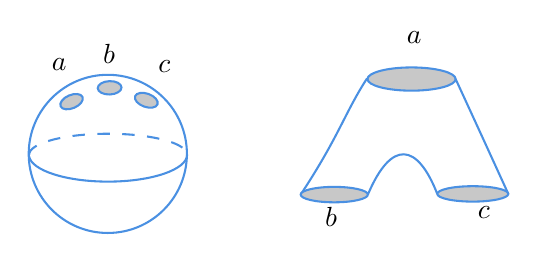
\begin{tikzpicture}[x=0.75pt,y=0.75pt,yscale=-1,xscale=1]
%uncomment if require: \path (0,109); %set diagram left start at 0, and has height of 109

%Shape: Arc [id:dp05657397073367365] 
\draw  [draw opacity=0][dash pattern={on 4.5pt off 4.5pt}] (215.19,65.11) .. controls (215.18,65.06) and (215.18,65.01) .. (215.18,64.96) .. controls (215.18,59.4) and (232.2,54.89) .. (253.18,54.89) .. controls (273.15,54.89) and (289.53,58.97) .. (291.07,64.16) -- (253.18,64.96) -- cycle ; \draw  [color={rgb, 255:red, 74; green, 144; blue, 226 }  ,draw opacity=1 ][dash pattern={on 4.5pt off 4.5pt}] (215.19,65.11) .. controls (215.18,65.06) and (215.18,65.01) .. (215.18,64.96) .. controls (215.18,59.4) and (232.2,54.89) .. (253.18,54.89) .. controls (273.15,54.89) and (289.53,58.97) .. (291.07,64.16) ;  
%Shape: Ellipse [id:dp11579635984986858] 
\draw  [color={rgb, 255:red, 74; green, 144; blue, 226 }  ,draw opacity=1 ] (214.97,64.6) .. controls (214.97,43.55) and (232.03,26.49) .. (253.08,26.49) .. controls (274.12,26.49) and (291.18,43.55) .. (291.18,64.6) .. controls (291.18,85.64) and (274.12,102.7) .. (253.08,102.7) .. controls (232.03,102.7) and (214.97,85.64) .. (214.97,64.6) -- cycle ;
%Shape: Arc [id:dp9816205265344173] 
\draw  [draw opacity=0] (291.3,64.82) .. controls (291.3,64.87) and (291.3,64.92) .. (291.3,64.96) .. controls (291.3,72.14) and (274.24,77.96) .. (253.18,77.96) .. controls (232.92,77.96) and (216.35,72.57) .. (215.14,65.77) -- (253.18,64.96) -- cycle ; \draw  [color={rgb, 255:red, 74; green, 144; blue, 226 }  ,draw opacity=1 ] (291.3,64.82) .. controls (291.3,64.87) and (291.3,64.92) .. (291.3,64.96) .. controls (291.3,72.14) and (274.24,77.96) .. (253.18,77.96) .. controls (232.92,77.96) and (216.35,72.57) .. (215.14,65.77) ;  
%Shape: Ellipse [id:dp6759124833295995] 
\draw  [color={rgb, 255:red, 74; green, 144; blue, 226 }  ,draw opacity=1 ][fill={rgb, 255:red, 200; green, 200; blue, 200 }  ,fill opacity=1 ] (230.33,41.65) .. controls (229.65,40.01) and (231.45,37.69) .. (234.37,36.46) .. controls (237.29,35.24) and (240.22,35.57) .. (240.9,37.21) .. controls (241.59,38.84) and (239.78,41.17) .. (236.87,42.39) .. controls (233.95,43.62) and (231.02,43.29) .. (230.33,41.65) -- cycle ;
%Shape: Ellipse [id:dp26656071826027805] 
\draw  [color={rgb, 255:red, 74; green, 144; blue, 226 }  ,draw opacity=1 ][fill={rgb, 255:red, 200; green, 200; blue, 200 }  ,fill opacity=1 ] (248.22,32.97) .. controls (248.16,31.2) and (250.67,29.66) .. (253.83,29.55) .. controls (257,29.43) and (259.62,30.78) .. (259.68,32.55) .. controls (259.75,34.33) and (257.23,35.86) .. (254.07,35.98) .. controls (250.91,36.09) and (248.29,34.75) .. (248.22,32.97) -- cycle ;
%Shape: Ellipse [id:dp4548290894023457] 
\draw  [color={rgb, 255:red, 74; green, 144; blue, 226 }  ,draw opacity=1 ][fill={rgb, 255:red, 200; green, 200; blue, 200 }  ,fill opacity=1 ] (266.22,36.83) .. controls (266.82,35.16) and (269.72,34.67) .. (272.7,35.73) .. controls (275.68,36.8) and (277.62,39.02) .. (277.02,40.7) .. controls (276.42,42.37) and (273.52,42.86) .. (270.53,41.79) .. controls (267.55,40.72) and (265.62,38.5) .. (266.22,36.83) -- cycle ;
%Curve Lines [id:da739129157041372] 
\draw [color={rgb, 255:red, 74; green, 144; blue, 226 }  ,draw opacity=1 ]   (345.99,84.21) .. controls (364.37,56.38) and (367.37,44.54) .. (377.99,28.21) ;
%Curve Lines [id:da8017147020708633] 
\draw [color={rgb, 255:red, 74; green, 144; blue, 226 }  ,draw opacity=1 ]   (446.04,83.88) .. controls (435.7,61.21) and (428.04,44.54) .. (420.66,28.54) ;
%Curve Lines [id:da5740408386448019] 
\draw [color={rgb, 255:red, 74; green, 144; blue, 226 }  ,draw opacity=1 ]   (378.37,84.21) .. controls (389.7,57.54) and (402.15,59.21) .. (411.81,83.88) ;
%Shape: Ellipse [id:dp32146447376371046] 
\draw  [color={rgb, 255:red, 74; green, 144; blue, 226 }  ,draw opacity=1 ][fill={rgb, 255:red, 200; green, 200; blue, 200 }  ,fill opacity=1 ] (378.18,28.54) .. controls (378.18,25.45) and (387.69,22.94) .. (399.42,22.94) .. controls (411.15,22.94) and (420.66,25.45) .. (420.66,28.54) .. controls (420.66,31.63) and (411.15,34.14) .. (399.42,34.14) .. controls (387.69,34.14) and (378.18,31.63) .. (378.18,28.54) -- cycle ;
%Shape: Ellipse [id:dp3365369220585279] 
\draw  [color={rgb, 255:red, 74; green, 144; blue, 226 }  ,draw opacity=1 ][fill={rgb, 255:red, 200; green, 200; blue, 200 }  ,fill opacity=1 ] (345.99,84.21) .. controls (345.99,82.16) and (353.24,80.49) .. (362.18,80.49) .. controls (371.12,80.49) and (378.37,82.16) .. (378.37,84.21) .. controls (378.37,86.26) and (371.12,87.93) .. (362.18,87.93) .. controls (353.24,87.93) and (345.99,86.26) .. (345.99,84.21) -- cycle ;
%Shape: Ellipse [id:dp6352897662304982] 
\draw  [color={rgb, 255:red, 74; green, 144; blue, 226 }  ,draw opacity=1 ][fill={rgb, 255:red, 200; green, 200; blue, 200 }  ,fill opacity=1 ] (411.81,83.88) .. controls (411.81,81.82) and (419.47,80.16) .. (428.92,80.16) .. controls (438.38,80.16) and (446.04,81.82) .. (446.04,83.88) .. controls (446.04,85.93) and (438.38,87.59) .. (428.92,87.59) .. controls (419.47,87.59) and (411.81,85.93) .. (411.81,83.88) -- cycle ;

% Text Node
\draw (224.66,17.29) node [anchor=north west][inner sep=0.75pt]    {$a$};
% Text Node
\draw (249.33,10.29) node [anchor=north west][inner sep=0.75pt]    {$b$};
% Text Node
\draw (275.99,17.95) node [anchor=north west][inner sep=0.75pt]    {$c$};
% Text Node
\draw (395.66,4.29) node [anchor=north west][inner sep=0.75pt]    {$a$};
% Text Node
\draw (356.33,88.72) node [anchor=north west][inner sep=0.75pt]    {$b$};
% Text Node
\draw (429.92,88.72) node [anchor=north west][inner sep=0.75pt]    {$c$};
\end{tikzpicture}
\caption{A three-times punctured sphere is known as a ``pair of pants”.}
\label{fig:pairOfPants}
\end{figure}


\begin{enumerate}
\item Write a general formula for the ground state degeneracy of an $M$-handled torus in terms of the $N$ matrices.
\item For the Fibonacci anyon model, find the ground state degeneracy of a 4-handled torus.
\item Show that in the limit of large number of handles $M$ the ground state degeneracy scales as $\sim \mathcal{D}^{2M}$ where $\mathcal{D}^{2} =\sum _{a}\mathrm{\mathsf{d}}_{a}^{2}$.
\end{enumerate}

\paragraph{Answer}



\section{Consistency of Fusion Rules}
Show by using commutativity and associativity of fusion along with identity \eqref{eq:timeReversalPropertyOfN}
\begin{equation}
N_{ab}^{c} =N_{\bar{a}\bar{b}}^{\bar{c}} ,
\label{eq:timeReversalPropertyOfN}
\end{equation}
that no anyon theory can have a particle $a$ such that $a\times a=a$ meaning $a$ fuses to $a$ to form only $a$ and nothing else.

\paragraph{Answer}
Suppose there is a theory that $a\times a=a$ and $a\neq I$, then consider the process of fusing $a,a$ and $\bar{a}$. We can simplicity, we can set the fusion rule between $a,\bar{a}$ is
\begin{equation}
a\times \bar{a} =I+c_{1} +\cdots +c_{n} .
\label{eq:fusionChannelOfaabar}
\end{equation}

As the Fig.\ref{fig:fusionOfThreeAnyons} shows, if we fuse $a\times a=a$ first, then fuse $a\times \bar{a}$, we will get $I+c_{1} +\cdots +c_{n}$ finally. However, if we change the order of fusion, fuse $a\times \bar{a}$ first and get $I+c_{1} +\cdots +c_{n}$, then fuse $a$, we will get 
\begin{equation*}
a\times \bar{a} =a+a\times c_{1} +\cdots +a\times c_{n} .
\end{equation*}
\begin{figure}[h!]
\centering
\tikzset{every picture/.style={line width=0.75pt}} %set default line width to 0.75pt        

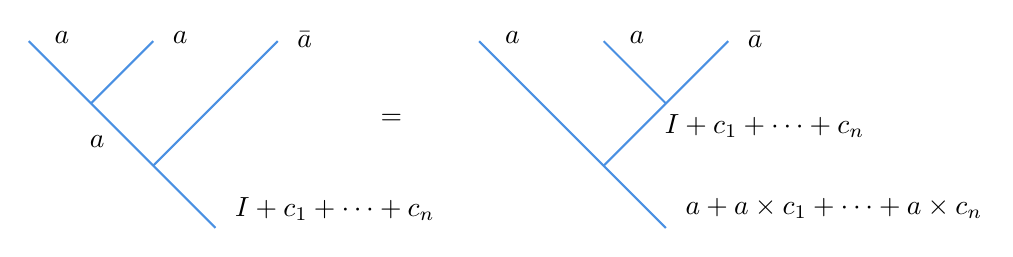
\begin{tikzpicture}[x=0.75pt,y=0.75pt,yscale=-1,xscale=1]
%uncomment if require: \path (0,100); %set diagram left start at 0, and has height of 100

%Straight Lines [id:da8590660242956558] 
\draw [color={rgb, 255:red, 74; green, 144; blue, 226 }  ,draw opacity=1 ]   (121,6) -- (211,96) ;
%Straight Lines [id:da4918681534713645] 
\draw [color={rgb, 255:red, 74; green, 144; blue, 226 }  ,draw opacity=1 ]   (151,36) -- (181,6) ;
%Straight Lines [id:da5778336776064139] 
\draw [color={rgb, 255:red, 74; green, 144; blue, 226 }  ,draw opacity=1 ]   (181,66) -- (241,6) ;

%Straight Lines [id:da5712783429115829] 
\draw [color={rgb, 255:red, 74; green, 144; blue, 226 }  ,draw opacity=1 ]   (338,6) -- (428,96) ;
%Straight Lines [id:da00547547016614347] 
\draw [color={rgb, 255:red, 74; green, 144; blue, 226 }  ,draw opacity=1 ]   (428,36) -- (398,6) ;
%Straight Lines [id:da2923856794370401] 
\draw [color={rgb, 255:red, 74; green, 144; blue, 226 }  ,draw opacity=1 ]   (398,66) -- (458,6) ;

% Text Node
\draw (289,40) node [anchor=north west][inner sep=0.75pt]    {$=$};
% Text Node
\draw (132,0) node [anchor=north west][inner sep=0.75pt]    {$a$};
% Text Node
\draw (189,0) node [anchor=north west][inner sep=0.75pt]    {$a$};
% Text Node
\draw (249,0) node [anchor=north west][inner sep=0.75pt]    {$\bar{a}$};
% Text Node
\draw (149,50) node [anchor=north west][inner sep=0.75pt]    {$a$};
% Text Node
\draw (219,80) node [anchor=north west][inner sep=0.75pt]    {$I+c_{1} +\cdots +c_{n}$};
% Text Node
\draw (349,0) node [anchor=north west][inner sep=0.75pt]    {$a$};
% Text Node
\draw (409,0) node [anchor=north west][inner sep=0.75pt]    {$a$};
% Text Node
\draw (466,0) node [anchor=north west][inner sep=0.75pt]    {$\bar{a}$};
% Text Node
\draw (426,40) node [anchor=north west][inner sep=0.75pt]    {$I+c_{1} +\cdots +c_{n}$};
% Text Node
\draw (436,80) node [anchor=north west][inner sep=0.75pt]    {$a+a\times c_{1} +\cdots +a\times c_{n}$};


\end{tikzpicture}
\caption{The fusion of $a,a,\bar{a}$.}
\label{fig:fusionOfThreeAnyons}
\end{figure}

In order to get the same result, we know that $\{a,a\times c_{1} ,\cdots ,a\times c_{n}\}$ must be a permutation of $\{I,c_{1} ,\cdots ,c_{n}\}$, which means $a\times c_{i}$ \textbf{cannot have multiple fusion channels} because each fusion channel have at least one result. Furthermore, in first case, we have $I$ in the final result, so $\exists i$, s.t. $c_{i} =\bar{a}$. Now the rule that $a\times c_{i}$ cannot have multiple fusion channel contradicts with \eqref{eq:fusionChannelOfaabar}, so no anyon theory can have a particle $a$ such that $a\times a=a$.
